\documentclass{sig-alternate}
\usepackage{verbatim}
\usepackage{array}
\usepackage{caption}
\usepackage{subcaption}
\usepackage{amsmath}
\usepackage{booktabs}
\usepackage{multirow}
\setcounter{secnumdepth}{5}
\usepackage{pdfpages}
\usepackage{url}

\newcommand{\argmax}{\arg\!\max} 
\newtheorem{definition}{Definition}



\begin{document}
\sloppy
\numberofauthors{4}

\author{
Craig Willis$^{1,3}$, Mike Lambert$^{1,3}$, Kenton McHenry$^{1,3}$, and Christine Kirkpatrick$^{2,3}$\\
     \affaddr{$^1$National Center for Supercomputing Applications, University of Illinois at Urbana-Champaign}\\     
     \affaddr{$^2$San Diego Supercomputer Center, University of California, San Diego}\\     
     \affaddr{$^3$National Data Service}\\     
     \email{\{willis8, lambert8, mchenry\}@illinois.edu, christine@sdsc.edu}
}
\CopyrightYear{}
\crdata{}
\permission{}
\copyrightetc{}
\conferenceinfo{}{}

\title{Container-based Analysis Environments for Low-Barrier Access to Research Data}

\maketitle
\begin{abstract}

The growing size of high-value sensor-born or computationally derived scientific datasets are pushing the boundaries of traditional models of data access and discovery. Due to their size, these datasets are often accessible only through the systems on which they were created. Access for scientific exploration and reproducibility is limited to file transfer or by applying for access to the systems used to store or generate the original data, which is often infeasible. There is a growing trend toward providing access to large-scale research datasets in-place via container-based analysis environments. This paper describes the National Data Service (NDS) Labs Workbench platform and DataDNS initiative. The Labs Workbench platform is designed to provide scalable and low-barrier access to research data via container-based services. The DataDNS effort is a new initiative designed to enable discovery, access, and in-place analysis for large-scale data, providing a suite of interoperable services to enable researchers, as well as the tools they are most familiar with, to access and analyze these datasets where they reside.

\end{abstract}

% A category with the (minimum) three required fields
\category{H.3.3}{Information Systems}{Computing Platforms}

%\terms{}
\keywords{Research data; Container-based analysis environments}

\section{Introduction}

Sensor-based, research-computing, and high-performance computing (HPC) systems now produce massive amounts of data.  Traditional data publishing services, such as doain and institutional repositories, are not equipped to handle large-scale research datasets.  Increasingly, researchers are leaving their data on research computing infrastructure or turning to cloud-based services to facilitate sharing and re-use. However, research-computing and HPC centers are typically not prepared to support long-term storage and access, as is often required by publishers and funders, further disconnecting these research products from traditional discovery methods. New models of in-place publishing are needed to connect research computing and data publishing infrastructure to support discovery and access for re-use and reproducibility.

Institutional and domain repositories are beginning to support ``remote'' data publishing.  With this approach, researchers are responsible for arranging for data storage with best-effort preservation and datasets effectively published in-place. Researchers provide the repository with descriptive metadata including methods of access and are assigned a digital object identifier (DOI).  Under this model, users can discover these datasets and information about how to access them via traditional discovery mechanisms, such as data search engines. However, it is up to the researcher or site where the data is hosted to support methods of access.

Existing approaches to providing access to these hosted datasets are inefficient and often ineffective.  Typically, research-computing infrastructure has supported two basic models of data access: transfer and direct access to the hosting system.  Data transfer services, such as Globus Online~\cite{Foster11}, enable users to access these datasets by transferring them to local systems via GridFTP~\cite{Allcock05}.  However, in many cases, the datasets are too large to move or copy. In these cases, researchers can apply for access to the systems used to generate and store the original data, but access is often restricted and, if available, an application process is involved and time consuming.

Container-based analysis environments are emerging as a mechanism to provide low-barrier access to research data in-place.  Using container technology such as Docker, projects provide access to large datasets through custom analysis environments, such as Jupyter notebooks or Rstudio server.  Typically, remote users are able to register for an account via web-based interfaces that allow them to launch specialized, resource-constrained analysis environments to explore data in-place. Examples include SciServer \cite{Medvedev:2016:SCB:2949689.2949700}, yt Hub \cite{zuhone2016galaxy}, and the TERRA-REF Analysis Workbench \cite{willis_craig_2017_580057}.  These services indicate a growing need for new methods of accessing research data, in partcilar where large datasets are involved, perhaps hosted in close proximity to computing infrastructure.

This paper describes two initiatives of the National Data Service consortium (NDS) to facilitate in-place access to large research datasets. The Labs Workbench platform, used by the U.S. Department of Energy Advanced Research Projects Agency - Energy (ARPA-E) TERRA Reference Data and Computing (TERRA-REF) project, is designed to support access to research data management and analysis tools via customizable container-based environments.  The second initiative, the DataDNS initiative is intended to connect various container-based analysis systems to the traditional publishing and discovery platforms to enable discovery, access, and analysis of datasets where they reside.

%\item There are lots of examples of low-barrier access being provided via Docker containers (yt.hub, SciServer, Whole Tale, Galaxy Portal, TERRA-REF, etc).
%\item Amazon public datasets
%\end{enumerate}

%Skyport
%Gerlach:2014:SCE:2689676.2689680
%http://dx.doi.org/10.1109/DataCloud.2014.6

This paper is organized as follows.  Section 2 provides a description of container-based analysis environments.  In Section 3 we describe the NDS Labs Workbench system and specifically how it's being used for the ARPA-E TERRA-REF project, followed by a description of the NDS DataDNS initiative in Section 4 and next steps in Section 5.

%\section{Research in the Cloud}

%TODO: It would be good to connect container-based environments to trends in cloud-computing for research computing.  This includes %services such as Amazon Public Datasets.
% https://scholar.google.com/scholar?hl=en&q=amazon+public+datasets&btnG=&as_sdt=1%2C14&as_sdtp=

\section{Container-based analysis environments}

Container technology is increasingly used in research computing as an alternative to hypervisor-based virtual machines for the packaging, deployment, and execution of software. Containers are considered to be more resource-efficient, provide a clear and light-weight abstraction for packaging, and are increasingly seen as a possible solution for the preservation of research software \cite{Meng2015137}.  Because of this, container management platforms such as Docker\footnote{\small http://www.docker.com} and rkt\footnote{\small https://coreos.com/rkt} have achieved widespread adoption. This section focuses on container use for access to research data. For more information about container technology, the reader is directed to more detailed analysis in \cite{7036275,7095802,Soltesz:2007:COS:1272998.1273025}. 

\emph{Container-based analysis environments} refer to systems that leverage container technology for the packaging and execution of interactive scientific research software. Containers are currently used in a variety of systems providing interactive and non-interactive access to research data. Systems such as SciServer, yt Hub, Whole Tale \cite{ludaescher2016capturing}, and the TERRA-REF Analysis Workbench provide interactive containerized environments based on software including Jupyter \cite{kluyver2016jupyter}, RStudio \cite{Rstudio2015}, and MATLAB \cite{mathworks}. Other systems, such as CyVerse\cite{devisetty2016bringing} and SciPort\cite{Gerlach:2014:SCE:2689676.2689680}, leverage containers for the management and execution of scientific workflows. We refer to these non-interactive environments as \emph{container-based execution environments}, which are more likely to fit into workflow systems and batch-scheduling infrastructure.  

Increasingly, research systems developers are seeing the need to support the computational research lifecycle from preliminary exploration through development and execution either on dedicated cloud-based or HPC systems. Container-based analysis environments support the early stages of exploratory analysis and development, while container-based execution environments serve as a bridge to traditional batch-compute systems.

\section{Labs Workbench}

Labs Workbench is an open-source platform developed by the National Data Service Consortium (NDSC) to facilitate sharing, discovery, evaluation, and development of research data management and analysis tools. The platform leverages Docker containers and the Kubernetes container orchestration framework to provide turn-key access to community developed tools. 

Labs Workbench has been effectively used in classroom and workshop environments to provide consistent, web-based access to applications \cite{ndsphenome}. In early 2017, the Labs Workbench was deployed by the ARPA-E TERRA-REF project to provide customized interactive analysis environments for the TERRA-REF reference dataset. 

\subsection{Use Case: TERRA-REF}

The ARPA-E TERRA program is focused on cutting-edge techniques for the improvement of biofuel crops in part through the creation and publication of a large public reference dataset, TERRA-REF, and associated compute pipeline \cite{arpae2015}. The TERRA-REF data storage and computing system will provide researchers with access to over 2PB of raw sensor and derived data hosted on the NSF ROGER system and made available via Globus, Clowder~\cite{Marini10,Sophocleous17}, BETYdb\footnote{\small https://www.betydb.org}, and the Labs Workbench. Researchers can also apply for accounts on the ROGER system directly for access via batch-processing. The TERRA-REF team is working with the Dryad data repository\footnote{\small https://www.datadryad.org} to publish the remotely-hosted reference dataset.

In early 2017, the TERRA-REF team used the Labs Workbench platform to host a workshop\footnote{\small http://www.phenome2017.org}, enabling ~50 participants to explore the reference dataset using domain-specific Jupyter, Rstudio and other interactive environments. Shortly after, an instance of Labs Workbench, named the TERRA-REF Analysis Workbench, was deployed on the National Center for Supercomputing Applications (NCSA) Nebula cloud-computing system to provide ongoing access to the TERRA-REF data for project contributors. Custom containers were created based on Jupyter, Rstudio, and other services to include dependencies required to access and use the TERRA-REF data such as NetCDF/NCO and OpenCV libraries~\cite{Kaebler}.  Additional containers were created to support system development, including a Python IDE for Clowder extractors and PostgresSQL Studio to provide access to the BETYdb PostGIS database.

The Labs Workbench platform was later used to support the two-week Program for Interdisciplinary and Industrial Internships at Illinois (PI4) Computational Mathematics Bootcamp\footnote{\small https://pi4-uiuc.github.io/2017-bootcamp}, an NSF funded program for graduate students to gain computational skills needed in scientific and engineering research labs. Students were provided with access to the TERRA-REF containers and data for a series of tutorials.

The TERRA-REF Analysis Workbench demonstrates that the same system can be used to provide access to data products for scientific exploration and reuse; collaborative system development; as well as education and training. To date, the system has been used to provide access to the TERRA-REF data for over 100 users, including system developers, researchers, students, and workshop participants.


\subsection{System architecture}

The Labs Workbench platform is based on the Kubernetes\footnote{\small http://www.kubernetes.io} container orchestration framework, deployed using the OpenStack\footnote{\small http://www.openstack.org} virtualization platform. Figure \ref{fig.arch} illustrates the basic architecture. First, a set of virtual machines and volumes is provisioned via the OpenStack API. Second, Kubernetes core services (controller, kubelet, and etcd) are deployed on each node. Third, Labs Workbench core and system services are deployed via Kubernetes. Labs Workbench core services include the Nginx ingress load-balancer (nginx-ilb), which provides authenticated access to running containers in the cluster, as well as a thin REST API server (ndslabs-apiserver) an Angular user interface (ndslabs-webui). System services include standard logging, monitoring and alerting (LMA) tools such as Kibana/ElasticSearch, Grafana/Heapster, and Nagios.  The system includes a private Docker registry for image caching.  Via Labs Workbench, users can launch a variety of Docker-based applications including but not limited to Jupyter and RStudio environments. The service catalog itself is a set of customizable Javascript Object Notation (JSON) objects currently stored in Github\footnote{https://www.github.com/nds-org/ndslabs-specs}. The Labs Workbench platform uses Gluster\footnote{https://www.gluster.org/} to provide shared storage between nodes and containers. Additional shared network volumes can also be mounted via other network services, such as NFS.

\begin{figure}[!ht]

\includegraphics[width=8.75cm]{architecture.png}
\caption{Labs Workbench systems architecture}
\label{fig.arch}
\end{figure}

\begin{figure}[!ht]
\frame{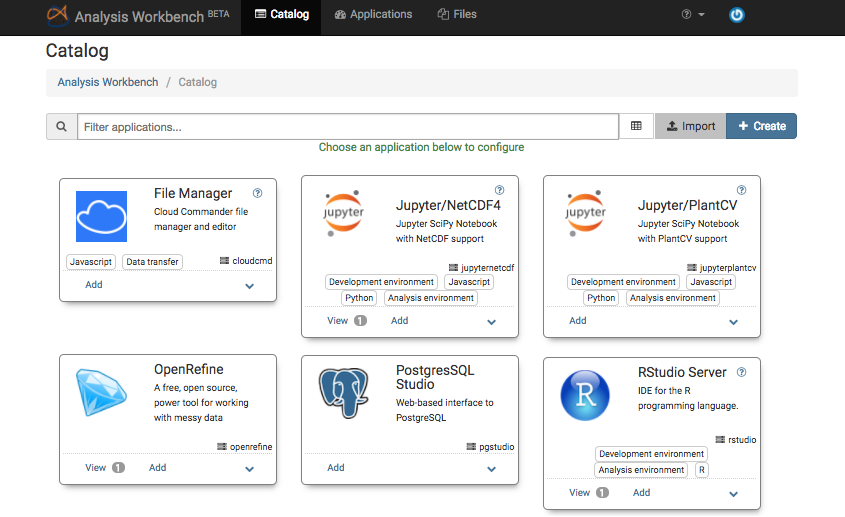
\includegraphics[width=8.75cm]{terraref-ui.png}}\\
\\
\frame{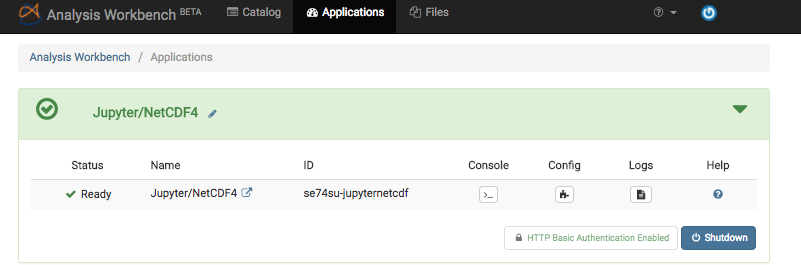
\includegraphics[width=8.75cm]{terraref-ui-apps.png}}
\caption{TERRA-REF Analysis Workbench catalog and application dashboard}
\label{fig.ui}
\end{figure}

The Labs Workbench system includes the following features:
\begin{enumerate}
\itemsep-0.2em
\item Catalog of community-contributed tools and services
\item Support for custom tools and personal catalogs
\item Dependency manamgment
\item Authentication
\item Logging and monitoring
\item Shared filesystem via GlusterFS
\item Scalable container orchestration
\end{enumerate}

The Labs Workbench user interface is presented in Figure \ref{fig.ui}.  The platform focused primarily on interactive, web-based applications including complex applications with multiple dependencies. Support is also available for command-line applications via web-based IDEs or terminal emulators.  

\section{DataDNS: A New Initiative}

The Labs Workbench is just one example of an emerging trend to provide access to research data via cloud and container-based environments.  Other examples include the SciServer Compute system which provides access to astronomy, materials science, turbulence, and earth science datasets via domain-specific Rstudio, MATLAB and Jupyter containers \cite{Medvedev:2016:SCB:2949689.2949700}.  More recently, yt Hub \cite{zuhone2016galaxy} uses the Girder data management platform\footnote{https://github.com/girder/girder} and custom Jupyter analysis environments to enable access to data for a number of fields including astronomy and cosmology. The yt Hub architecture is currently being adapted to support the Whole Tale project \cite{ludaescher2016capturing}, and the Renaissance Simulations Laboratory (RSL), providing access to large-scale astrophysics simulations \cite{2041-8205-807-1-L12}.

\begin{figure}[!ht]
\frame{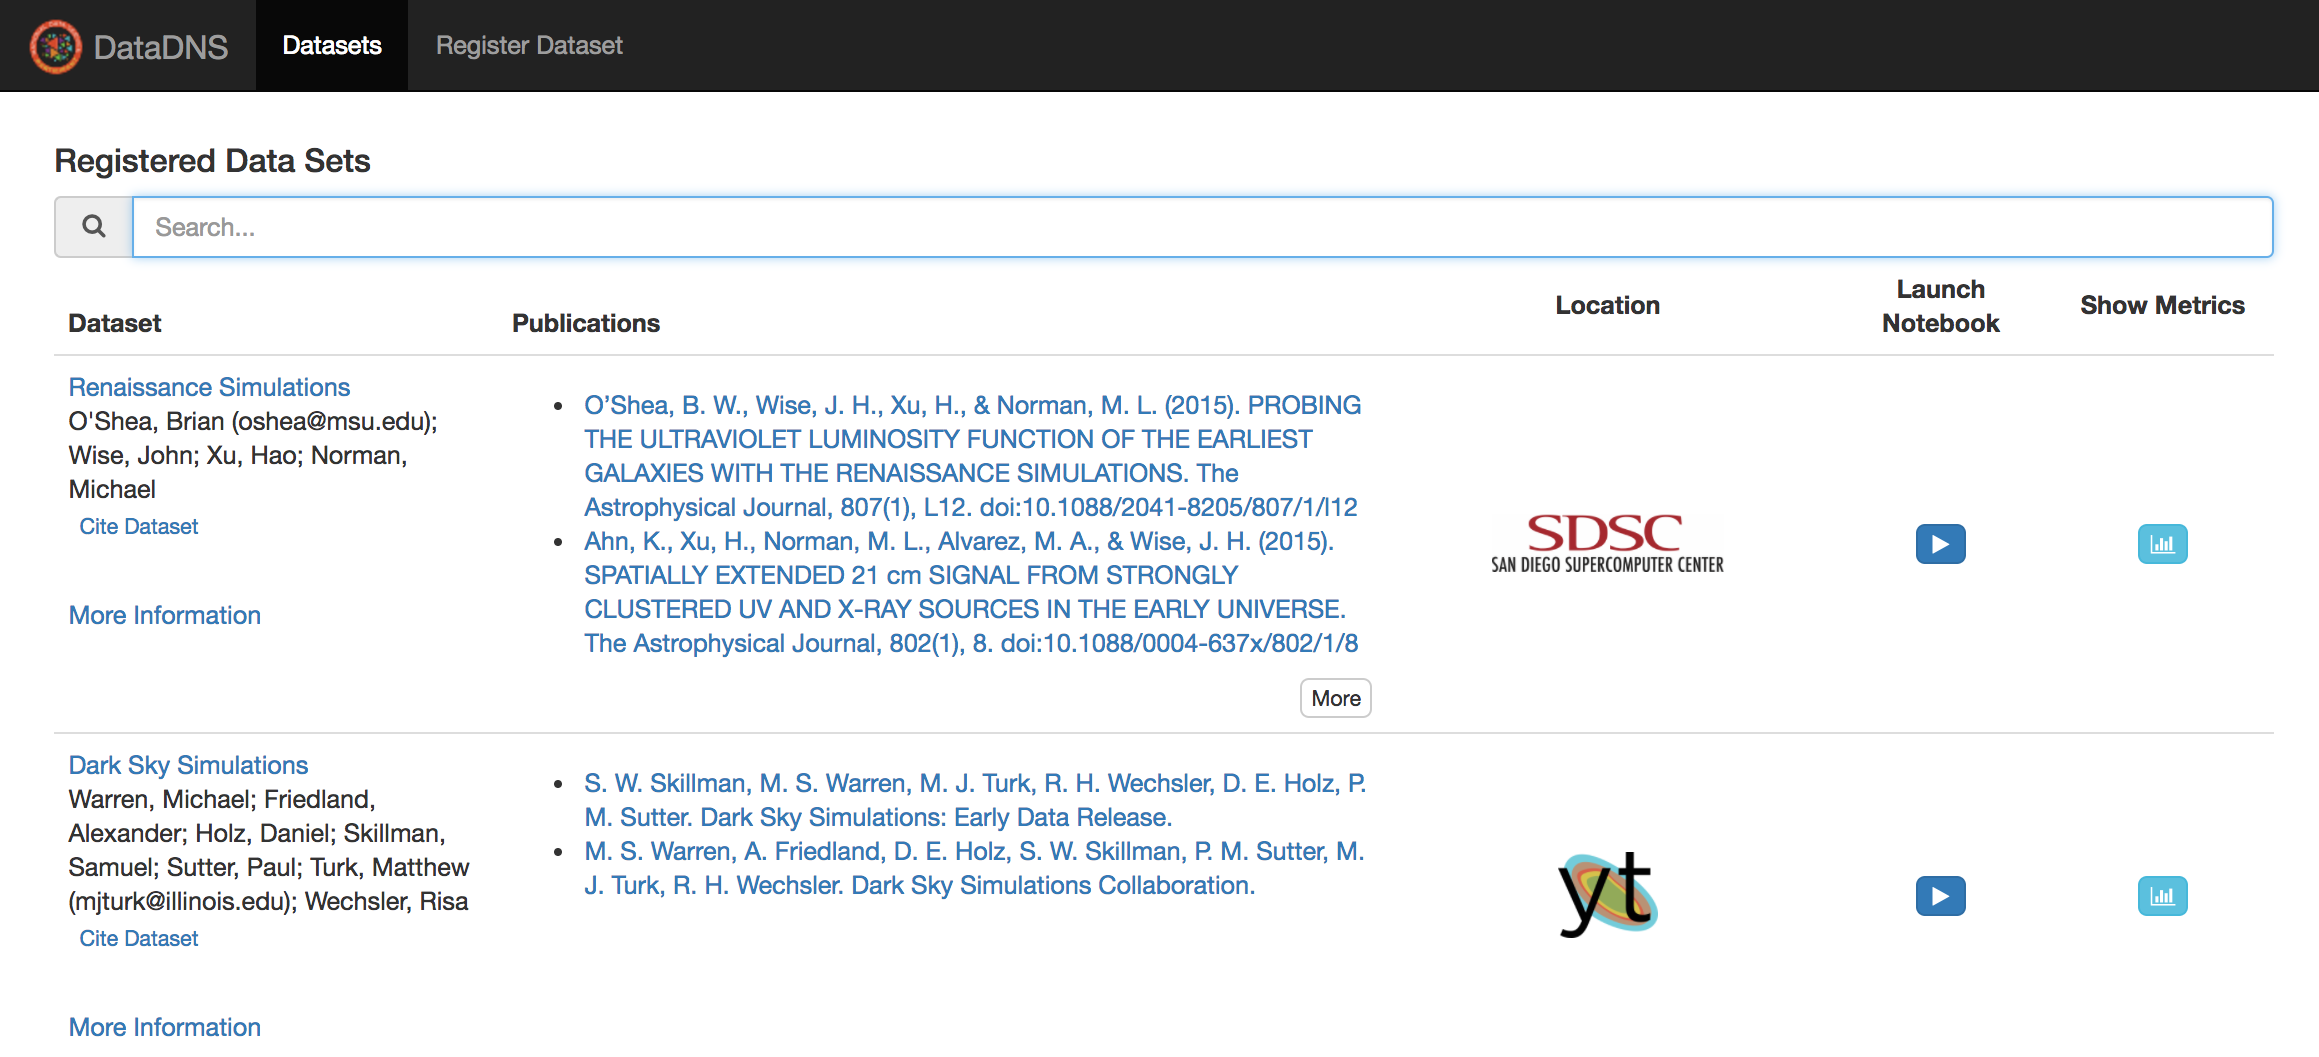
\includegraphics[width=8.75cm]{datadnsui.png}}\\
\vspace{-0.1in}
\caption{DataDNS prototype search interface}
\label{fig.datadns}
\end{figure}

While container-based analysis environments enable new forms of access to research data, they do not yet connect to data publishing and discovery tools.  The DataDNS initiative, still in the early stages of development, will leverage container-enabled analysis environments and other capabilities of research computing platforms to enable discovery, access, and in-place analysis of data.  This will be achieved through an active registry and resolution service that tracks the locations and capabilities associated with remotely hosted datasets. Capabilities include file transfer or container-based, cloud-based or batch compute. Through existing data discovery services, such as domain repositories or search engines, researchers will not only be able to discover these datasets, but also their physical locations allowing them to access and launch remote analysis, when possible.   

Figure \ref{fig.datadns} presents the DataDNS prototype search interface. Through this interface, the user can both discover available datasets as well as launch analysis at the remote hosting site. This functionality will be exposed via an API, allowing other systems to offer similar functionality.

As an example, we can consider the yet-to-be published TERRA-REF reference dataset. The dataset is hosted on the ROGER system, which includes access via Globus (data transfer), Analysis Workbench (container-enabled compute), OpenStack (dedicated virtual machines), and batch compute cluster.  Metadata describing the reference dataset is published with the Dryad data repository and exposed via the DataCite search engine\footnote{http://search.datacite.org}. Through DataDNS and the tracked location/resource information, a user who discovers the dataset via these systems would be able to launch an analysis environment via the Analysis Workbench, transfer the data, or apply for access to dedicated and batch compute resources.


\section{Conclusions and Next Steps}

Traditional data publishing service, such as community and institutional repositories, are not equipped to handle publication of or access to very large research datasets.  Container-based analysis environments, such as Labs Workbench, provide a scalable, resource constrained, and low-barrier approach to providing access to data hosted on research computing and HPC systems. These services open up  new opportunities to support access to large-scale data.  DataDNS will connect these and other compute-centric resources to traditional discovery methods, such as institutional and community repositories, to further enable re-use of remotely hosted data.

Development of the Labs Workbench platform and DataDNS system are ongoing.  Upcoming features include support for commercial cloud services, distributed/federated deployments, single sign-on, and overall a simplified installation processes. We are also working on improved support for mounting external data into the system and exploring approaches to supporting job scheduling and execution.

\bibliographystyle{abbrv}
\small
\bibliography{containers}  


\end{document}
